\section{Theory}

\subsection{Analog circuit}
\label{sec:analogCircuit}
The analog circuit has input signals delivered by the digital circuitry, and delivers its output to two ADCs. The analog circuit diagram is given in figure \ref{fig:analogCircuit}, where each of the four pixel block has the circuit given in figure \ref{fig:pixelCircuit}.

\begin{figure}[H]
    \centering
    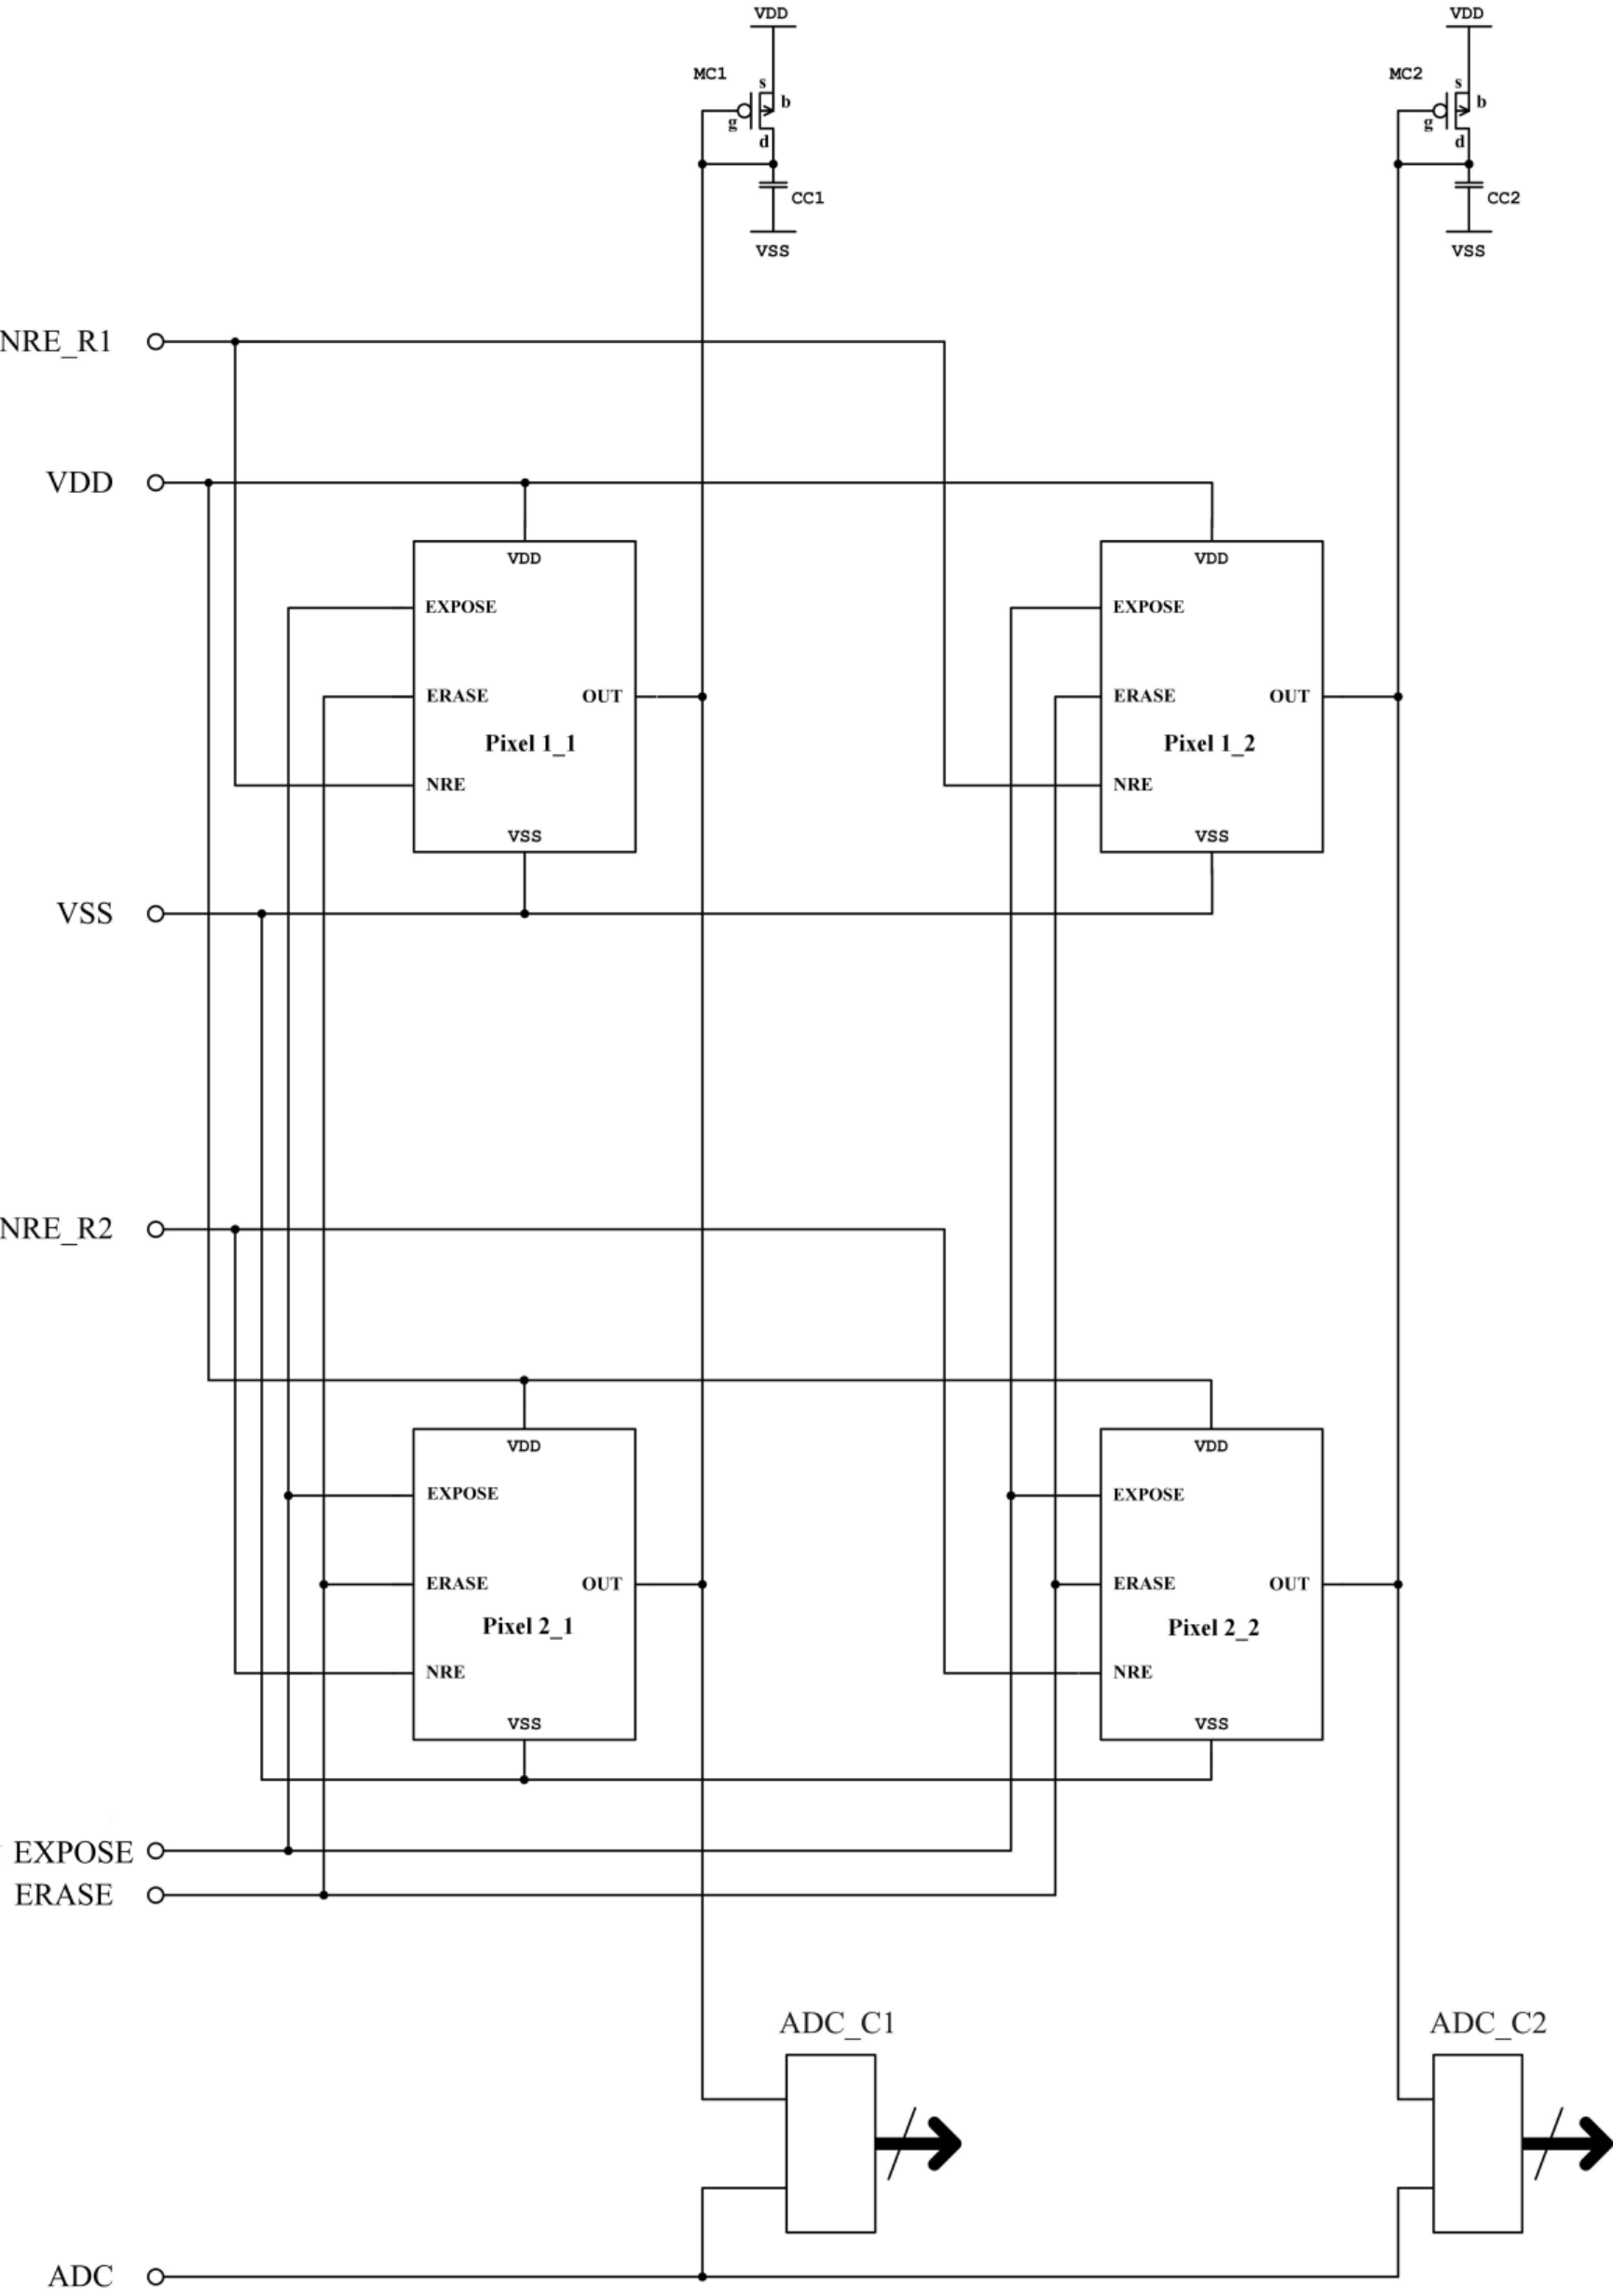
\includegraphics[width=0.8\textwidth]{graphs/analogCircuit.png}
    \caption{Analog circuit schematic.}
    \label{fig:analogCircuit}
\end{figure}

\begin{figure}[H]
    \centering
    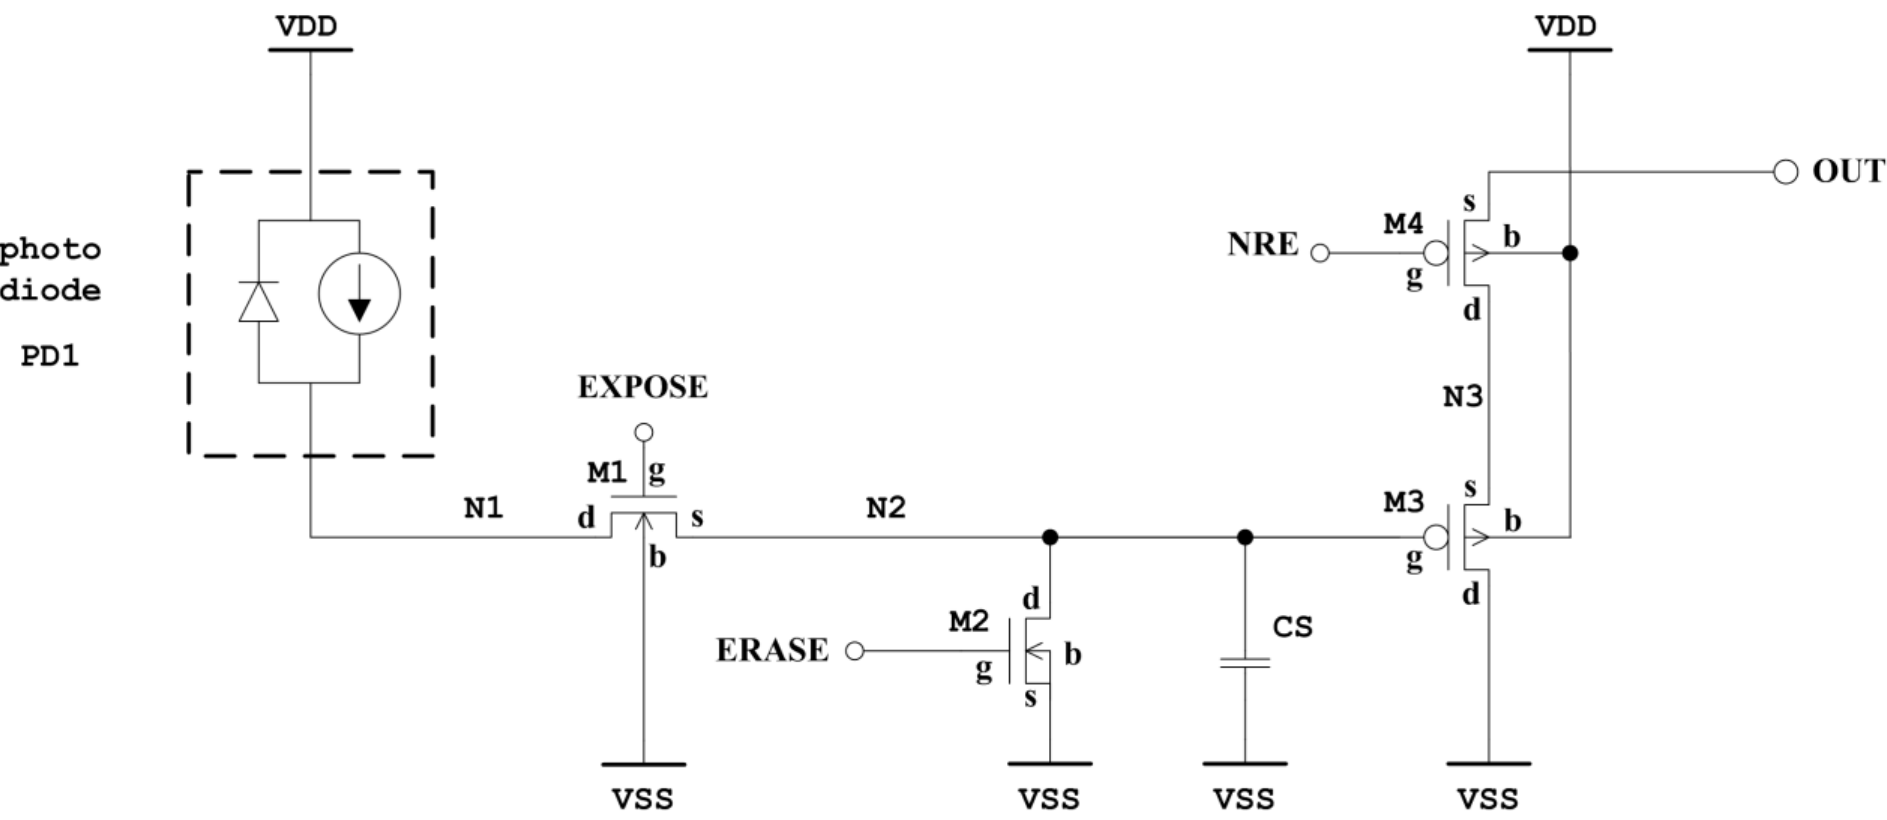
\includegraphics[width=\textwidth]{graphs/pixelCircuit.png}
    \caption{Pixel cicuit schematic.}
    \label{fig:pixelCircuit}
\end{figure}

In detail, the analog circuit consists of 4 pixels in a 2x2 array. Each pixel in the same row shares the same \emph{NRE} (Not-REad) input which means they are sending data to the ADC at the same time. Each pixel in the same column share the same active load and readout wire, which means they need to send data to the ADC at different times.

\subsubsection{Conceptual operation of pixel circuit}

Schematics for the pixel circuit is given in figure \ref{fig:pixelCircuit}. It consists of a photo diode PD1, three switch transistors M1, M2 and M4, one buffer transistor M3 and a charge storage capacitor $C_S$. The photo diode is modeled by a diode and an ideal current source in parallel. The current source outputs a current $I_D$ that is proportional to the illumination intensity on that particular pixel. This current is used to charge the transistor $C_S$. Ideally, we want that all of $I_D$ flows through M1 and into $C_S$ when \emph{EXPOSE} is \verb|HIGH| and all of $I_D$ flows back through the diode in the photo diode model when \emph{EXPOSE} is \verb|LOW|. In that way the voltage on node N2 when \emph{EXPOSE} has been \verb|HIGH| for a time $t$ is given by

\begin{equation}
    V_{CS}(t) = \frac{1}{C_S} \int_0^t I_D(t) dt.
\end{equation}

This means the voltage $V_{CS}$ is proportional to the total illumination on the pixel throughout the exposure time, which is exactly what we want.

But since the camera is supposed to be reusable, we need a way to erase that charge before taking a new picture. That is what M2 is for. Ideally we want M2 to be a perfect switch, so that when \emph{ERASE} is \verb|HIGH|, $C_S$ is instantly uncharged through M2 and when \emph{ERASE} is \verb|LOW|, M2 does not conduct any current at all.

For the readout we do not want to connect N2 directly to OUT, since the output wire might be very long and have a big capacitance. Instead, the voltage $V_{CS}$ controls the conductance through a transistor M3. The higher $V_{CS}$, the lower conductance through M3 and higher voltage on OUT. In that way, the current required to control the voltage on the output wire is supplied through the active load in the top of each output wire, outside the pixel circit.

But since all pixels in the same column share the same output wire we need a way to unconnect N3 from OUT, and that is what M4 is for. M4 is supposed to be an ideal switch so that the pixel is driving OUT only when \emph{NRE} is \verb|LOW|.

\subsubsection{Dimensions for switch transistors}
\label{sec:switch_dimensions}
The transistors M1, M2 and M4 all function as switches, where a digital gate input decides whether the transistor should act as a short-circuit between drain and source, or as an open circuit. Since these transistors simply should have two possible states, it is key that the leakage current is minimized. This is particularly important for M1 and M2 to ensure that the voltage over $C_s$ is as constant as possible during readout. In \emph{Analog Circuit Design} by Tony Chan Carusone, one can read in section 1.4.1 that the subthreshold leakage current is given by

\begin{equation}
    \label{eq:leakage}
    I_{off} = (n-1) \mu_n C_{ox} \left( \frac{W}{L} \right) \left( \frac{kT}{q} \right)^2 \exp{(-qV_t / nkT)}.
\end{equation}

In order to minimize this leakage current, $\frac{W}{L}$ need to be as small as possible, meaning the smallest possible width $W$ and the largest possible length $L$ is desired. The technology used will limit the possible width and length of the transistor, thus $W$ and $L$ can be chosen accordingly.

\subsubsection{Value for $C_s$}

To choose a suitable value for $C_s$ spice simulations can be used. To know what values are the best we will look at the four corner cases for exposure time and light conditions. The corner cases will be denoted exposure-light, so for example max-min is maximum exposure time and minimum light. The voltage over $C_S$ after exposure in each corner will get different values for different values of $C_S$. There are many possible approaches to how these corners should be tuned, and the one that we will apply is the following:

\begin{itemize}
    \item Max-max corner should make $C_s$ fully charged.
    \item Min-min corner should leave $C_s$ uncharged.
    \item Min-max and max-min corners should make $C_s$ half full charged.
\end{itemize}

The reason for why we want the corners to be like that is beyond the scope of this report.

\subsubsection{Values for M3 and active load}

\begin{figure}[H]
    \centering
    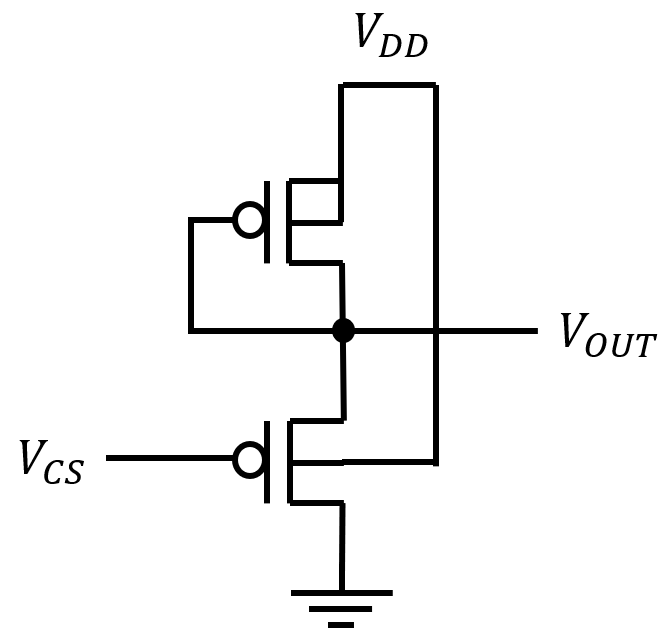
\includegraphics[width=0.5\textwidth]{graphs/m3AndActiveLoad.png}
    \caption{Simplified schematic for output voltage driving circuit.}
    \label{fig:m3AndActiveLoad}
\end{figure}

Values for M3 and active load should be tuned for maximum dynamic range, but it will not have a very big impact since it is a very robust and self-regulating system. If we assume $C_{C1}$ and $C_{C2}$ are very small, the output system can be simplified to figure \ref{fig:m3AndActiveLoad}. Essentially, the output voltage $V_{OUT}$ depends on how the conductance in the uppermost and downmost transistor are relative to each other. These conductances are proportional to $W/L$ in the transistors and they also vary with the gate-source voltages. To avoid unnecessary simplifications, it is best to decide these $W/L$-ratios from SPICE-simulations. The dynamic range is the difference between the output voltage when uncharged and fully charged, and it is preferable that it is as big as possible.

\subsubsection{Process variations}

It is important to look at how process variations will impact an analog design. One way to do this is to look at the what is called FF, FS, SF and SS corners. F means fast, S means slow, the first letter is for NMOS and the second is for PMOS. For this design it is enough to look at how the switch transistors are affect by process variations. The values to measure in each corner is $R_{DS}$ when switched off and on.

For curiosity we will also have a look at how these two corners affect the analog circuit as a whole.

\subsection{Digital camera controller}
The digital input signals in the analog circuit need to be controlled by a digital circuit - the digital camera controller. The module interface for the digital camera controller is described in the figure below.

\begin{figure}[H]
    \centering
    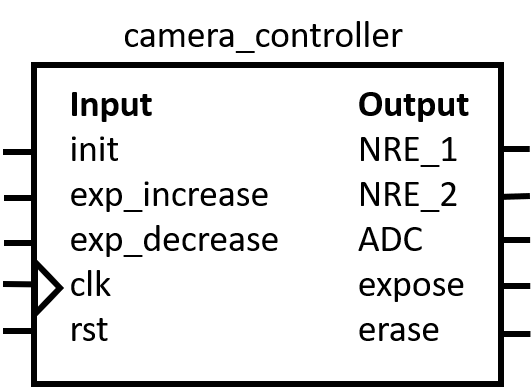
\includegraphics[width=0.4\textwidth]{graphs/camera_controller_pinout.png}
    \caption{Overview of input and output pins for the camera controller module.}
    \label{fig:io}
\end{figure}

It has inputs \emph{init}, \emph{exp\_increase}, \emph{exp\_decrease}, \emph{clk} and \emph{rst}. \emph{clk} is controlled by an internal camera module, while the four other signals are controlled by the user. \emph{init} is \verb|HIGH| when the user presses the shutter button, \emph{exp\_increase} is \verb|HIGH| when the user wants to increase the exposure time, \emph{exp\_decrease} is \verb|HIGH| when the user wants to decrease the exposure time (and is overridden by \emph{exp\_increase} if they conflict, i.e. if they are \verb|HIGH| at the same time), and \emph{rst} is \verb|HIGH| when the user wishes to cancel any ongoing process, or reset the exposure time.

The outputs are \emph{NRE\_1}, \emph{NRE\_2}, \emph{ADC}, \emph{EXPOSE} and \emph{ERASE}, all of which were described in section \ref{sec:analogCircuit}.

\subsubsection{Finite state machine}
\label{sec:fsm}
The wanted behaviour of the digital camera controller is described in the finite state machine (FSM) in figure \ref{fig:fsm}.

\begin{figure}[H]
    \centering
    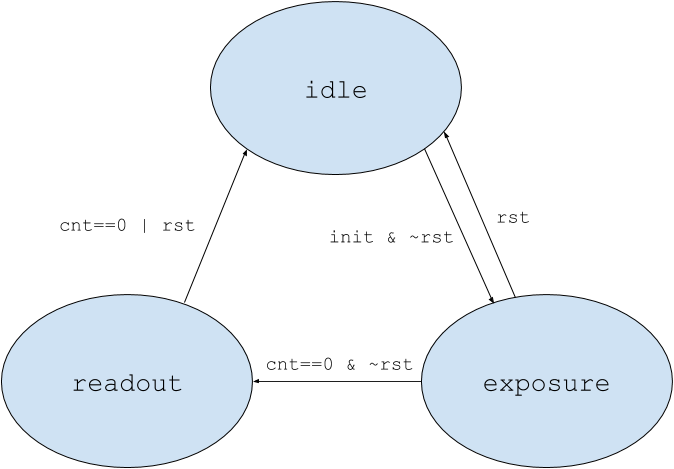
\includegraphics[width=\textwidth]{graphs/fsm.png}
    \caption{The finite state machine for the digital camera controller.}
    \label{fig:fsm}
\end{figure}

In the FSM, there are three states. The camera starts in the \emph{idle} state. In this state, the camera isn't in the process of taking any picture, so output signals \emph{EXPOSE} and \emph{ADC} should be \verb|LOW|, and \emph{NRE\_1} and \emph{NRE\_2} should be \verb|HIGH|. The camera should also prepare itself for a new picture in this state, so \emph{ERASE} should be \verb|HIGH| to erase any voltage from the potential previous exposure. The user should be able to adjust the exposure time with the signals \emph{exp\_increase} and \emph{exp\_decrease} in the \emph{idle} state. These signals will respectively increase or decrease the exposure time with $1$ms for each clock cycle they're \verb|HIGH| to a minimum of $2$ms and a maximum of $30$ms. When the signal \emph{init} is \verb|HIGH|, the camera will enter the \emph{exposure} state. The exception is if the \emph{rst} input signal is \verb|HIGH|. In any state, \emph{rst} being \verb|HIGH| should override any process and take the camera back to \emph{idle}.

When the camera is entering the \emph{exposure} state, \emph{ERASE} should be set \verb|LOW| and \emph{EXPOSE} should be set \verb|HIGH| to begin the exposure. If \emph{rst} is \verb|HIGH| at any time during \emph{exposure}, the camera should return to the \emph{idle} state. When the preset exposure time has passed, the camera should enter the \emph{readout} state if \emph{rst} is \verb|LOW|. Exposure being finished is called \emph{exp\_done} in figure \ref{fig:fsm}.

The \emph{readout} state is the final state, in which the data from the individual pixels are read and inputted in the ADC. First, \emph{EXPOSE} should be set \verb|LOW| since the exposure is done. Then, \emph{NRE\_1} should be \verb|LOW| first at the same time as \emph{ADC} is \verb|HIGH|, to read from the top two pixels and input it to the ADC. Lastly, \emph{NRE\_2} should be \verb|LOW| at the same time as \emph{ADC} is \verb|HIGH| to do the same for the bottom two pixels. Exactly how the output signals should be will be properly explored in the next section. When the readout sequence is finished, called \emph{ro\_done} in figure \ref{fig:fsm}, the camera should enter the \emph{idle} state again. As with the \emph{exposure} state, \emph{rst} being \verb|HIGH| at any time should return the camera to \emph{idle}. It is important that the camera stays in \emph{idle} for at least one clock cycle before the user is able to take another picture, to ensure that the data of the previous photo is erased.

\subsubsection{Output timing}

The desired time chartis illustrated in figure \ref{fig:timechart}.

\begin{figure}[H]
    \centering
    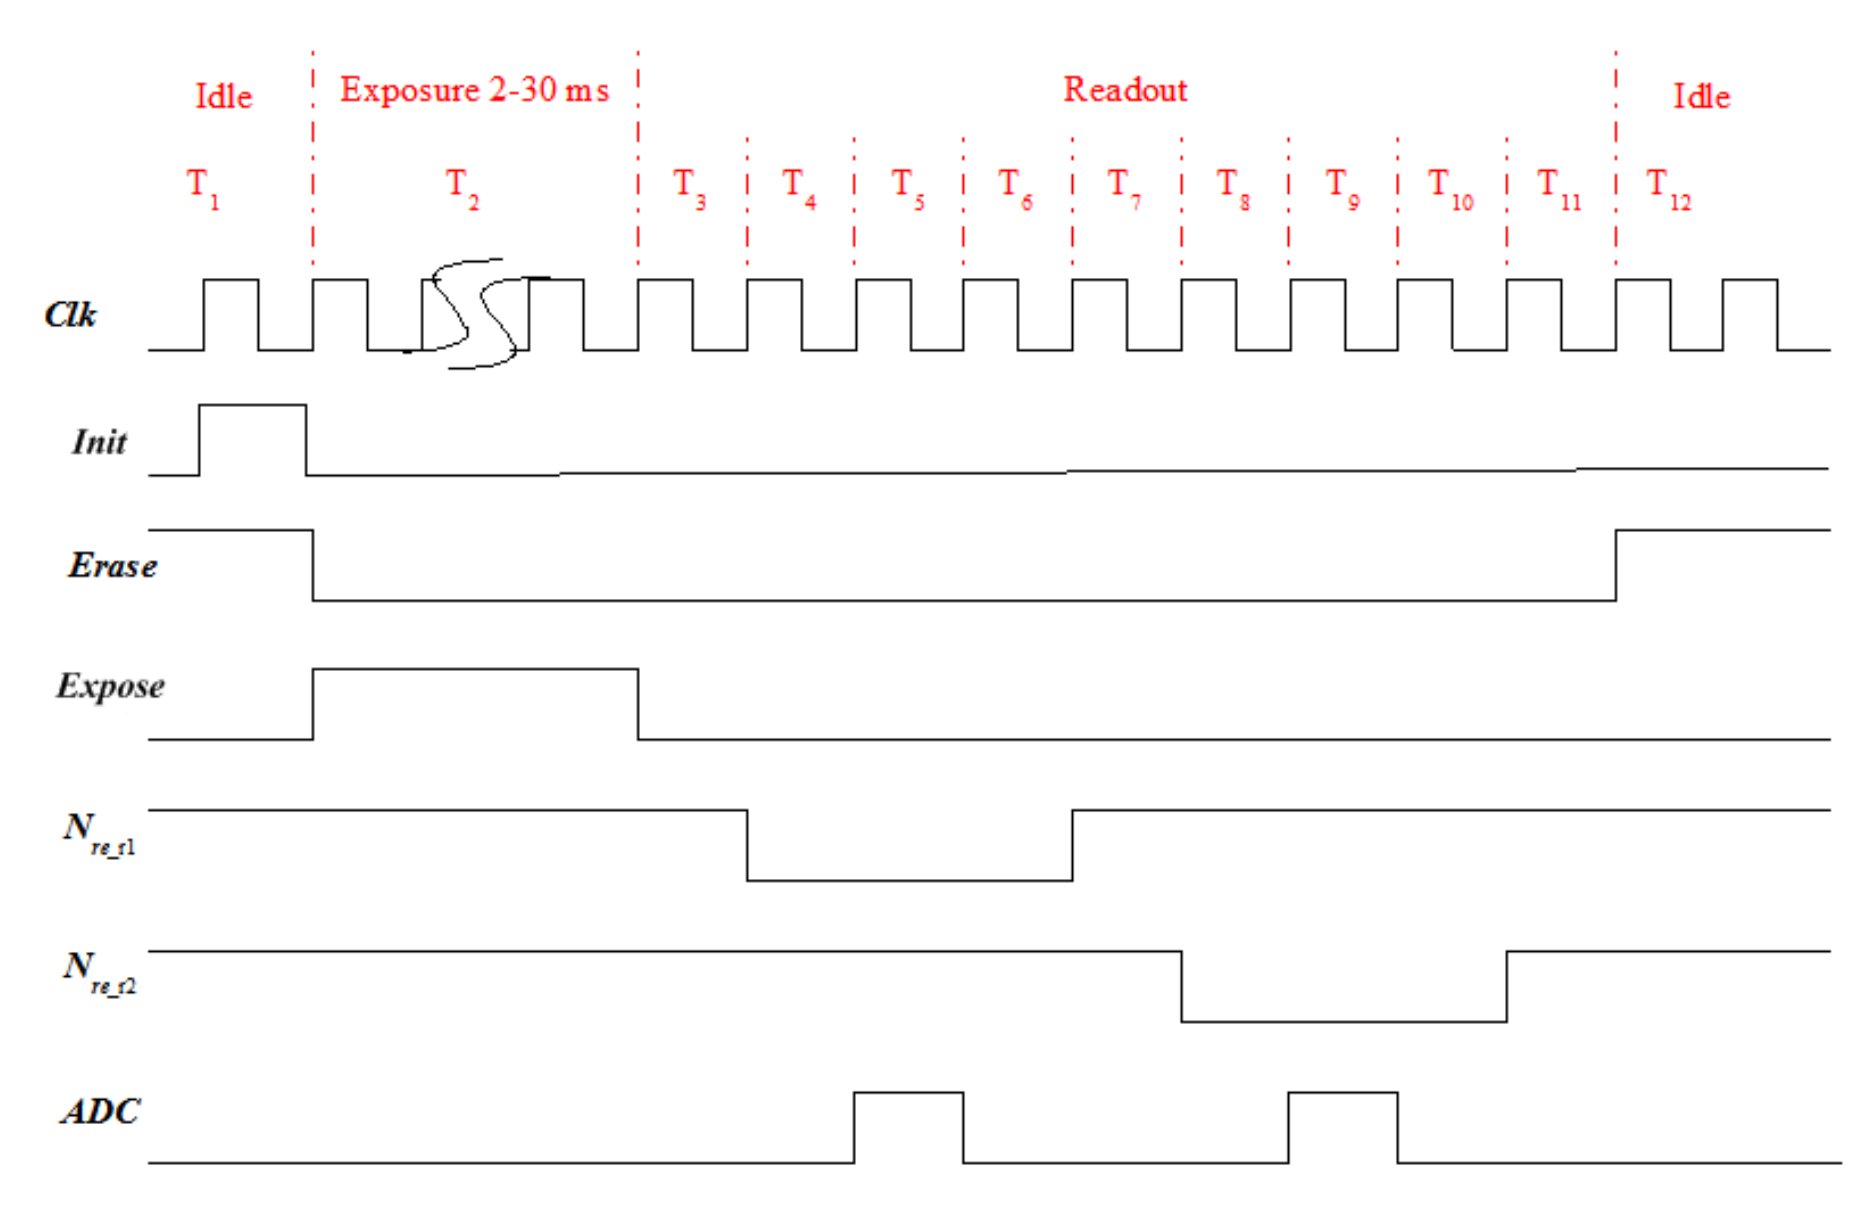
\includegraphics[width=\textwidth]{graphs/time_chart.png}
    \caption{The desired time chart for the output signals of the digital camera controller.}
    \label{fig:timechart}
\end{figure}

In the \emph{idle} state and \emph{exposure} state, the output signals are as described in the previous subsection. Notably, \emph{ERASE} is \verb|HIGH| during \emph{idle} and \emph{EXPOSE} is \verb|HIGH| during \emph{exposure}. The \emph{readout} state is more complex, as output signals are altered in every clock cycle. In the first cycle, $T_3$ in the figure, \emph{EXPOSE} is set \verb|LOW| to end exposure before readout begins. From $T_4$ to $T_6$, \emph{NRE\_1} is set \verb|LOW|, with \emph{ADC} being \verb|HIGH| in the middle $T_5$. This is to ensure that \emph{NRE\_1} is not transienting from \verb|HIGH| to \verb|LOW| or \verb|LOW| to \verb|HIGH| while the ADC is reading. In $T_7$, \emph{NRE\_1} is set \verb|HIGH| again. From $T_8$ to $T_{10}$, the reading process repeats for \emph{NRE\_2} to read the bottom two pixels. In the last clock cycle of the state, $T_{11}$, \emph{NRE\_2} is set \verb|HIGH| again to end the readout. It can be noted that the \emph{readout} state has a fixed duration of $9$ clock cycles, as the only state with a fixed duration.
